%\documentclass[journal=jctcce,manuscript=article]{achemso}
\documentclass[11pt,oneside,a4paper]{article}
\usepackage[T1]{fontenc}
\usepackage{graphicx}
\usepackage{amsmath,amssymb,mathrsfs}
%\usepackage{xr}
\usepackage{booktabs}
\usepackage{multirow}
\usepackage{siunitx}
\usepackage{easy-todo}
%\usepackage{footref}
%\externaldocument[S-]{SI}

\sisetup{
  separate-uncertainty = true
}

\renewcommand{\footnoterule}{}
\renewcommand{\vec}[1]{\mathbf{#1}}


\title{Reaction field derivation}

%\input{affiliations}

%\keywords{Free Energy, Hydration, Alchemical, Reproducibility, Automation}



\begin{document}

%\begin{abstract}

%\end{abstract}


%\section{Introduction}
%\label{sec:intro}


\section{Onsager reaction field}
\label{sec:onsager}

In order to correctly derive a charge--dipole interaction in a reaction field, I will follow the approach used by Onsager ~\cite{onsager1936electric} for a reaction field of a dipole in a cavity of radius $a$.
The initial hypotheses are: 
\begin{itemize}
 \item The dipole is rigid and its shape do not influence the electrostatic potential
 \item The dipole moment is $\mu$
 \item the dipole can be thought as a singularity in the center of the cavity
 \item the cavity is immersed in a uniform dielectric material, with dielectric constant $\epsilon_1$
\end{itemize}


\begin{figure}[h!]
\caption{Onsager system~\cite{onsager1936electric}:a rigid single-point dipole in a cavity (yellow) or radius $a$, immersed in a uniform dielectric (blue) $\epsilon_1$.\label{fig:cavityOnsager}}
 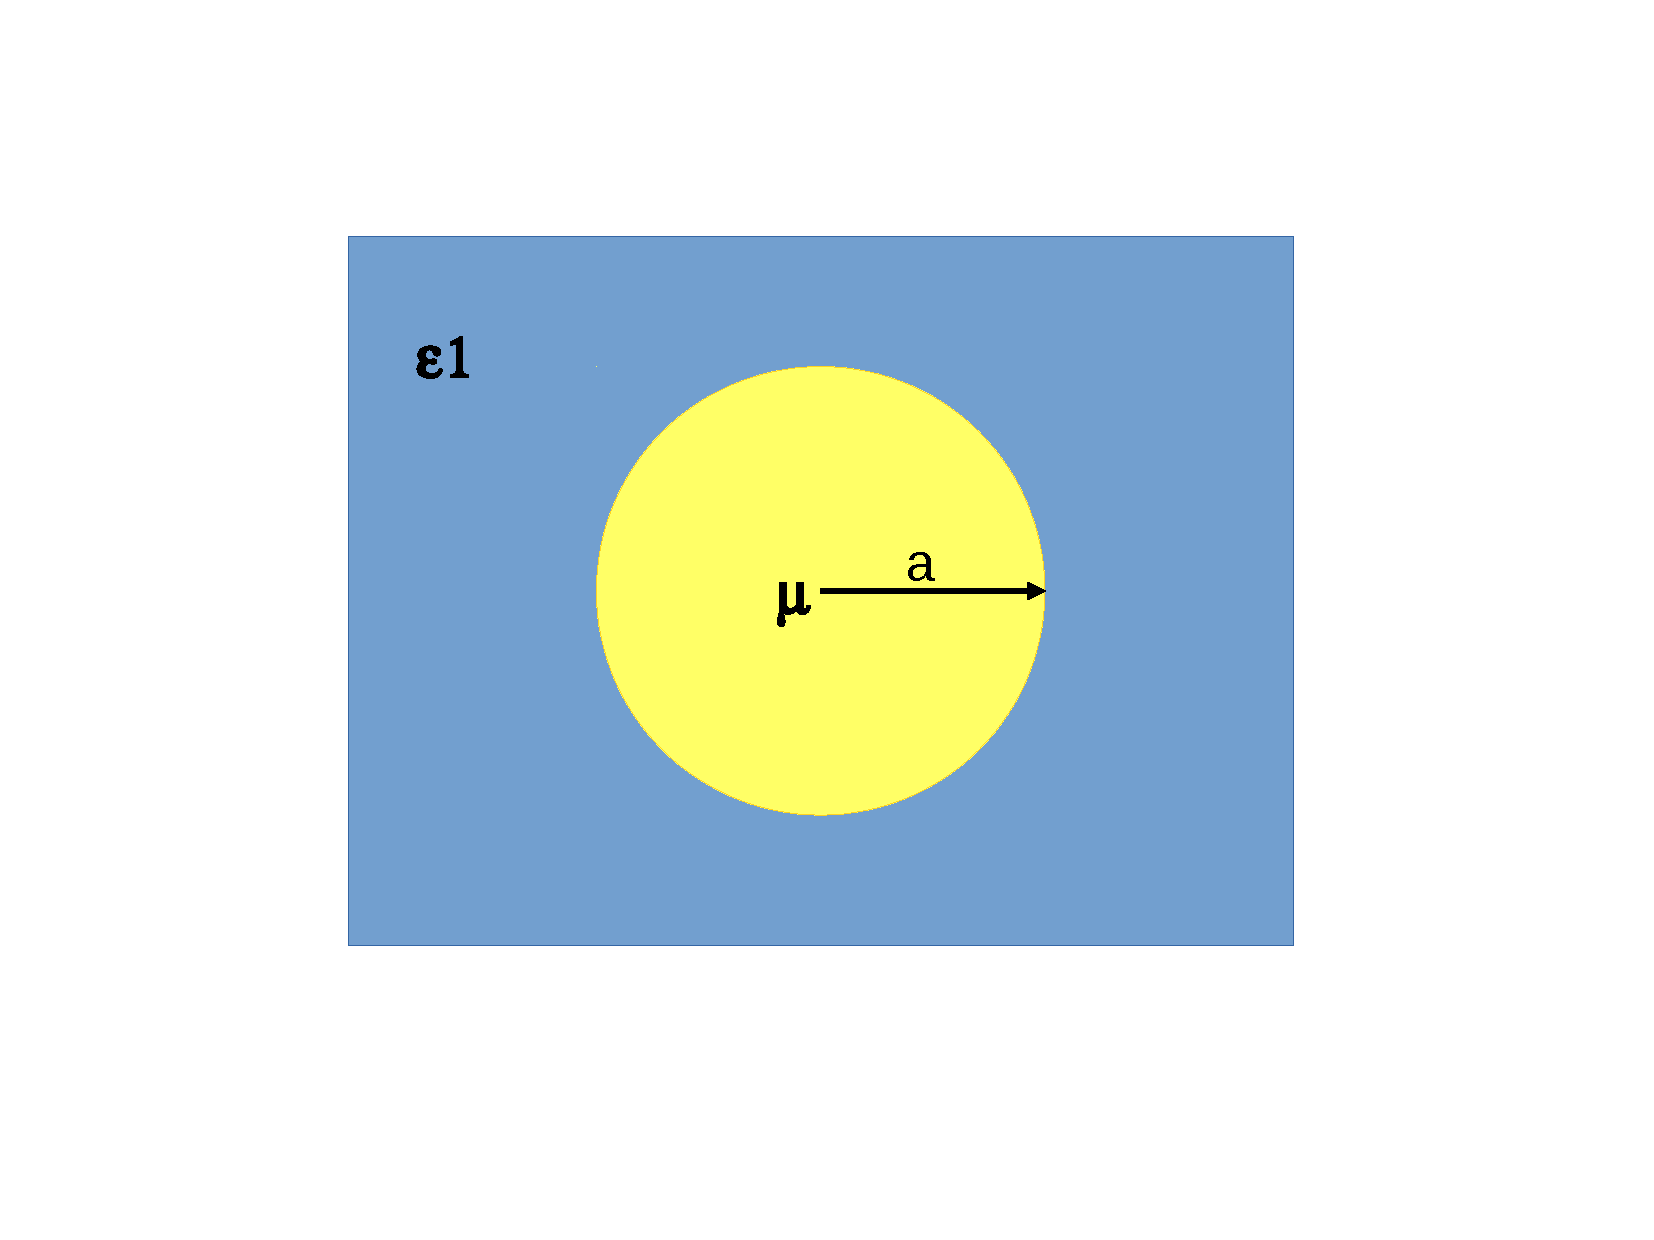
\includegraphics[width=\textwidth]{figures/Onsager.pdf}
 \centering
\end{figure}

Fig.~\ref{fig:cavityOnsager} shows the system under study. The total electrostatic potential $\psi(\mathbf{r})$, as a function of the vector position $\mathbf{r}$, must satisfy the Laplace equation all around the system: 
\begin{equation}
\label{eq:laplace}
\Delta \psi(\mathbf{r}) = 0
\end{equation}

Passing to polar coordinates, eq.~\ref{eq:laplace}  can be solved with the technique of separation of variables :
\begin{equation}
 \label{eq:separation}
 \psi(\mathbf{r},\mathbf{\theta}) = R(\mathbf{r})\Theta(\mathbf{\theta})
\end{equation}
where $R(\mathbf{r})$ is a function depending on the coordinates only  and $\Theta(\mathbf{\theta})$ depends on the rotational degree of freedom $\mathbf{\theta}$. 
A known solution for $R(\mathbf{r})$ and $\Theta(\mathbf{\theta})$ is based on the use of spherical harmonics, giving a final potential $\psi(\mathbf{r},\mathbf{\theta})$ : 
\begin{equation}
 \label{eq:generalsolution}
 \psi(\mathbf{r},\mathbf{\theta}) = \sum_{l=0}^{\infty} \left ( A_{l} \mathbf{r}^{l} +  \frac{B_{l}}{\mathbf{r}^{l+1}} \right )  P_{l}(\cos\theta)
\end{equation}
where the sum is extended to all the $l$th-term, $A_{l}$ and $B_{l}$ are constants to be determined with the boundary conditions and $P_{l}$ is the $l$th Legendre polynomial. 
From this general solution, we can express the electrostatic potential $\psi(\mathbf{r},\mathbf{\theta})$ as a sum of internal cavity potential $\psi_\mathrm{in}(\mathbf{r},\mathbf{\theta})$ and dielectric medium potential $\psi_\mathrm{out}(\mathbf{r},\mathbf{\theta})$, which must satisfy the following conditions:
\begin{equation}
\begin{cases}
 \lim_{\mathrm{r\to 0}} \psi_\mathrm{in}(\mathbf{r},\mathbf{\theta}) &= \frac{\mu\cos\theta}{4\pi\epsilon_0 r^2}\\
 \\
 \lim_{\mathrm{r\to \infty}} \psi_\mathrm{out}(\mathbf{r},\mathbf{\theta}) &=  0
\end{cases}
\end{equation}
where $\mu$ is the dipole moment and $\frac{\mu\cos\theta}{4\pi\epsilon_0 r^2}$is the dipole electrostatic potential, where $\epsilon_0$ is the vacuum permittivity. Thus, $\psi_\mathrm{in}(\mathbf{r},\mathbf{\theta})$ and  $\psi_\mathrm{out}(\mathbf{r},\mathbf{\theta})$ can be expressed as a general solution from eq.~\ref{eq:generalsolution} as:
\begin{equation}
 \label{eq:psiinpsiout}
 \begin{align} 
 \psi_\mathrm{in}(\mathbf{r},\mathbf{\theta}) &= \frac{\mu \cos\theta}{4\pi\epsilon_0 r^2} + \sum_{l=0}^\infty A_{l} r^{l}P_{l}(\cos\theta) \\
 \\
 \psi_\mathrm{out}(\mathbf{r},\mathbf{\theta}) &= \sum_{l=0}^\infty \frac{B_{l}}{r^{l+1}} P_{l}(\cos\theta) 
  \end{align}
\end{equation}
 
Futhermore, the following conditions hold at the boundary of the spherical cavity surface:
\begin{itemize}
 \item The potential is continuous across the boundary:
 \begin{equation}
  \label{eq:boundary1}
  \psi_\mathrm{in}(a)  = \psi_\mathrm{out}(a) 
 \end{equation}
 \item The normal component of the dielectric displacement across the surface is continuous:
 \begin{equation}
  \label{eq:boundary2}
 \frac{\partial \psi_\mathrm{in}}{\partial \mathbf{r}} = \epsilon_1 \frac{\partial \psi_\mathrm{out}}{\partial \mathbf{r}} 
 \end{equation}
\end{itemize}
where position and angular dependency was omitted for ease of notation.
Now, from eq.~\ref{eq:boundary1} a set of equations can be obtained:
\begin{equation}
 \label{eq:boundary1solved}
 \begin{cases}
  \frac{\mu\cos\theta}{4\pi\epsilon_0 a^2} + A_1 a^1 \cos\theta = \frac{B_1}{a^2}\cos\theta   & \mbox{if } l=1 \\
  \\
  A_{l}a^{l} = \frac{B_{l}}{a^{l+1}} &\mbox{if } l\ne 1
 \end{cases}
\end{equation}
which can be solved as:
\begin{equation}
 \label{eq:boundary1solved2}
 \begin{cases}
  B_1 & = \frac{\mu}{4\pi\epsilon_0} + A_1 a^3 \\
  \\
  B_{l} &= (a^{2l + 1} )A_{l}
 \end{cases}
\end{equation}
Thus, from the conditions ~\ref{eq:boundary2}, the electric displacement is:
\begin{equation}
 \label{eq:boundary2solved}
 \begin{cases}
  -\frac{\mu}{2\pi\epsilon_0 a^3} + A_1  & = -\frac{2\epsilon_1}{a^3}B_1  \\
  \\
  A_{l} l a^{l-1} &  = -\epsilon_1 (l+1) \frac{B_{l}}{a^{l+2}} 
 \end{cases}
\end{equation}
Substituting eq.~\ref{eq:boundary1solved2} into eq.~\ref{eq:boundary2solved} :
\begin{equation}
\label{eq:boundary2solved2}
\begin{cases}
 A_1 &= \frac{\mu}{2\pi\epsilon_0 a^3}\left (\frac{1-\epsilon_1}{1+2\epsilon_1} \right ) \\
 \\
 A_{l} & = B_{l} = 0 
\end{cases} 
\end{equation}
From this solution it is possible to express $B_1$ :
\begin{equation}
 \label{eq:boundary2solved3}
 B_1 = \frac{\mu}{4\pi\epsilon_0}\left(\frac{3}{1+2\epsilon_0}\right)
\end{equation}

From eq.~\ref{eq:boundary2solved2} and ~\ref{eq:boundary2solved3} the final electrostatic potential can be expressed as:
\begin{equation}
\label{eq:finalpsi}
\begin{align} 
\psi_\mathrm{in}(\mathbf{r},\mathbf{\theta}) &= \frac{\mu\cos\theta}{4\pi\epsilon_0 r^2} \left\{ 1+ 2\frac{r^3}{a^3} \left ( \frac{1 - \epsilon_1}{1 + 2\epsilon_1} \right)  \right \} \\
\\
\psi_\mathrm{out}(\mathbf{r},\mathbf{\theta}) &= \frac{\mu\cos\theta}{4\pi\epsilon_0 r^2} \left ( \frac{3}{1 + 2\epsilon_1} \right ) 
 \end{align}
\end{equation}
giving $\psi(\mathbf{r},\mathbf{\theta})$ :
\begin{equation}
 \psi(\mathbf{r},\mathbf{\theta}) = \frac{\mu\cos\theta}{4\pi\epsilon_0 r^2}\left\{1 + 2\frac{r^3}{a^3}\left ( \frac{1 - \epsilon_1}{1 + 2\epsilon_1} \right ) + \left ( \frac{ 3}{1 + 2\epsilon_1} \right ) \right \}
\end{equation}

\section{Reaction field for a charge-dipole interaction}
\label{sec:chargedipole}

In this case in the cavity a charge $q_\mathrm{c}$ and a dipole $\mu$ are present. The charge--dipole electrostatic potential can be expressed as:
\begin{equation}
 \label{eq:chargedipoleint}
 V(\mathbf{r},\mathbf{\theta}) = -\frac{q_\mathrm{c}\mu\cos\theta}{4\pi\epsilon_0 r^2}
\end{equation}

Recalling eq.~\ref{eq:psiinpsiout}, the total electrostatic potential  $\psi(\mathbf{r},\mathbf{\theta})$ can be expressed as:
\begin{equation}
 \label{eq:qdpsiinpsiout}
 \begin{align} 
 \psi_\mathrm{in}(\mathbf{r},\mathbf{\theta}) &= -\frac{q_\mathrm{c}\mu \cos\theta}{4\pi\epsilon_0 r^2} + \sum_{l=0}^\infty A_{l} r^{l}P_{l}(\cos\theta) \\
 \\
 \psi_\mathrm{out}(\mathbf{r},\mathbf{\theta}) &= \sum_{l=0}^\infty \frac{B_{l}}{r^{l+1}} P_{l}(\cos\theta) 
  \end{align}
\end{equation}
which satisfies the following conditions:
\begin{equation}
\begin{cases}
 \lim_{\mathrm{r\to 0}} \psi_\mathrm{in}(\mathbf{r},\mathbf{\theta}) &= -\frac{q_\mathrm{c}\mu\cos\theta}{4\pi\epsilon_1 r^2}\\
 \\
 \lim_{\mathrm{r\to \infty}} \psi_\mathrm{out}(\mathbf{r},\mathbf{\theta}) &=  0
\end{cases}
\end{equation}

Again, for eq.~\ref{eq:qdpsiinpsiout} the boundary conditions expressed in ~\ref{eq:boundary1} and ~\ref{eq:boundary2} must hold. Applying the condition ~\ref{eq:boundary1} the following equations are obtained:
\begin{equation}
 \label{eq:qdboundary1solved}
 \begin{cases}
  -\frac{q_\mathrm{c}\mu\cos\theta}{4\pi\epsilon_0 a^2} + A_1 a^1 \cos\theta = \frac{B_1}{a^2}\cos\theta   & \mbox{if } l=1 \\
  \\
  A_{l}a^{l} = \frac{B_{l}}{a^{l+1}} &\mbox{if } l\ne 1
 \end{cases}
\end{equation}
which can be solved as:
\begin{equation}
 \label{eq:qdboundary1solved2}
 \begin{cases}
  B_1 & = -\frac{q_\mathrm{c}\mu}{4\pi\epsilon_0} + A_1 a^3 \\
  \\
  B_{l} &= (a^{2l + 1} )A_{l}
 \end{cases}
\end{equation}

From condition ~\ref{eq:boundary2} a new set of equations can be solved:
\begin{equation}
 \label{eq:qdboundary2solved}
 \begin{cases}
  \frac{q_\mathrm{c}\mu}{2\pi \epsilon_0 a^3} + A_1  & = -2\epsilon_1 \frac{B_1}{a^3}  \\
  \\
  \epsilon_1 A_{l} l a^{l-1} &  = -\epsilon_2 (l+1) \frac{B_{l}}{a^{l+2}} 
 \end{cases}
\end{equation}
\newpage

Eq.~\ref{eq:qdboundary2solved} brings to the solution for $A_1$, $B_1$ and $A_{l}$ and $B_{l}$ : 
\begin{equation}
\label{eq:qdboundary2solved2}
\begin{cases}
 A_1 &= \frac{q_\mathrm{c}\mu}{4\pi\epsilon_0 a^3}\left (\frac{\epsilon_1 -1}{1+2\epsilon_1}\right )  \\
 \\
 B_1 &=\frac{q_\mathrm{c}\mu}{2\pi\epsilon_0}\left ( -\frac{1}{2} + \frac{\epsilon_1 - 1}{1+2\epsilon_1} \right )  \\
 \\
 A_{l} = B_{l} & = 0
\end{cases} 
\end{equation}

Combining equations ~\ref{eq:qdboundary2solved2} into eq.~\ref{eq:qdpsiinpsiout}, $\psi_\mathrm{in}$ and $\psi_\mathrm{out}$ can be expressed as:
\begin{equation}
\label{eq:qdfinalpsi}
\begin{align} 
\psi_\mathrm{in}(\mathbf{r},\mathbf{\theta}) &= -\frac{q_\mathrm{c}\mu \cos\theta}{4\pi\epsilon_0}\left ( -\frac{1}{r^2} + 2 \frac{r}{a^3}\left ( \frac{\epsilon_1 -1}{1+2\epsilon_1} \right ) \right )  \\
\\
\psi_\mathrm{out}(\mathbf{r},\mathbf{\theta}) &= -\frac{q_\mathrm{c}\mu \cos\theta}{4\pi\epsilon_0 r^2} \left ( \frac{3}{1+2\epsilon_1} \right ) 
 \end{align}
\end{equation}

Finally, the total electrostatic potential $\psi(\mathrm{r},\mathbf{\theta})$ is:
\begin{equation}
\label{eq:rfpot}
 \psi(\mathbf{r},\mathbf{\theta}) = -\frac{q_\mathrm{c}\mu \cos\theta}{4\pi\epsilon_0}\left ( \frac{1}{r^2} -\frac{2r}{a^3}\frac{\epsilon_1 -1}{1 + 2\epsilon_1} + \frac{1}{r^2}\frac{3}{1 + 2\epsilon_1} \right )  
\end{equation} 


\section{Derivation of a rotationally-averaged charge-dipole reaction field potential}
\label{sec:rotavg}

Considering a charge-dipole system, the system's potential energy is influenced by the dipole rotations, described by an angle $\theta$. In particular, these rotations are about the dipole center and relative to the interacting charge $q_\mathrm{c}$.
To work out a single optimal value for the electrostatic potential charge-dipole interactions, a rotationally-averaged potential $\psi(\mathbf{r},\mathbf{\theta}) \rangle$  can be computed by employing the Boltzmann average, starting from the charge-dipole interaction, given in eq.~\ref{eq:rfpot}:
\begin{equation}
 \label{eq:boltzmannavg}
 \langle \psi(\mathbf{r},\mathbf{\theta}) \rangle = \frac{\int_{0}^{\pi} C \cos\theta e^{-\frac{C\cos\theta}{k_\mathrm{B}T}} \sin\theta d\theta } {\int_{0}^{\pi}e^{-\frac{C\cos\theta}{k_\mathrm{B}T}} \sin\theta d\theta} 
\end{equation}
where $C= -\frac{q_\mathrm{c}\mu}{4\pi\epsilon_0}\left ( \frac{1}{r^2} -\frac{2r}{a^3}\frac{\epsilon_1 -1}{1 + 2\epsilon_1} + \frac{1}{r^2}\frac{3}{1 + 2\epsilon_1} \right ) $ and $\sin\theta d\theta$ is the polar angular variable of integration.
The term $e^{-\cos\theta}$ cannot be carried out analytically, but it can be rewritten in terms of Taylor expansion as:
\begin{equation}
 \label{eq:taylorexp}
 e^{-\cos\theta} \sim 1 - \cos\theta
\end{equation}
So the integral in eq.~\ref{eq:boltzmannavg} simplifies as :
\begin{equation}
 \label{eq:simplification}
\langle \psi(\mathbf{r},\mathbf{\theta}) \rangle = \frac{\int_{0}^{\pi} C\cos\theta\sin\theta - C\cos\theta\sin\theta\frac{C\cos\theta}{k_\mathrm{B}T} d\theta}
{\int_{0}^{\pi} \sin\theta -\sin\theta\frac{C\cos\theta}{k_\mathrm{B}T} d\theta}
\end{equation}

Now, computing each multiplication and carrying out all the terms not depending on $\theta$, 4 integrals are obtained and can be solved. In particular, $\int_{0}^{\pi}\cos\theta\sin\theta d\theta=0$ since $\cos\theta\sin\theta$ is a symmetric function in $[0..\pi]$ and $\int_{0}^{\pi}\cos^2\theta\sin\theta d\theta$ can be computed by substitution, namely $\sin\theta=t$.

Plugging each solved integral in eq.~\ref{eq:simplification}, the final rotationally-averaged charged dipole reaction field integration is obtained:
\begin{equation}
 \label{eq:avgrot}
 \langle \psi(\mathbf{r}) \rangle  = -\frac{C^2}{3k_\mathrm{B}T}
\end{equation}
The $C$ term can be written as:
\begin{equation}
 \label{eq:cterm}
 C = -\frac{q_\mathrm{c}\mu}{4\pi\epsilon_0 r^2} \left ( 1 - 2\frac{r^3}{a^3}\left (\frac{\epsilon_1 -1}{1+2\epsilon_1} \right ) + \left (\frac{3}{1+2\epsilon_1} \right ) \right ) = A\left ( 1 - 2\frac{r^3}{a^3}\left ( \epsilon^\prime \right ) + \left (\epsilon^{\prime\prime} \right )    \right ) 
\end{equation}
where $A =-\frac{q_\mathrm{c}\mu}{4\pi\epsilon_0 r^2}$, $\epsilon^\prime = \frac{\epsilon_1 -1}{1+2\epsilon_1}$ and $\epsilon^{\prime\prime} = \frac{3}{1+2\epsilon_1}$. 
Computing $C^2$ gives:
\begin{equation}
 \label{eq:csquared}
 C^2 = A^2\left ( 1 + 4\frac{r^6}{a^6}{\epsilon^\prime}^2 + {\epsilon^{\prime\prime}}^2 - 4\frac{r^3}{a^3}\epsilon^\prime + 2\epsilon^{\prime\prime} - 4\frac{r^3}{a^3}\epsilon^\prime \epsilon^{\prime\prime} \right ) = A^2 \left(\left (\epsilon^{\prime\prime} + 1 \right)^2 + 4\frac{r^3}{a^3}\left ( \frac{r^3}{a^3}{\epsilon^\prime}^2 - \epsilon^\prime - \epsilon^\prime \epsilon^{\prime\prime} \right ) \right )
\end{equation}
The term $4\frac{r^3}{a^3}\left ( \frac{r^3}{a^3}{\epsilon^\prime}^2 - \epsilon^{\prime} - \epsilon^\prime \epsilon^{\prime\prime} \right ) $ can be solved as $4\frac{r^3}{a^3}\epsilon^\prime\left ( \epsilon^\prime \left (\frac{r^3}{a^3} - 2 \right ) -2\epsilon^{\prime\prime} \right ) $.
Thus, $C^2$ can be written as:
\begin{equation}
\label{eq:cterm2}
C^2 = \left (\frac{q_\mathrm{c}\mu}{4\pi\epsilon_0 r^2} \right )^2 \left( 4(\epsilon^\prime + \epsilon^{\prime\prime})^2 + 4\frac{r^3}{a^3}\epsilon^\prime \left( \epsilon^\prime \left (\frac{r^3}{a^3} - 2 \right ) -2\epsilon^{\prime\prime} \right) \right ) 
\end{equation}

Finally, the rotationally-averaged charge dipole reaction field potential is:
\begin{equation}
 \label{eq:rotavgpot}
 \langle \psi(\mathbf{r}) \rangle = -\frac{1}{3k_\mathrm{B}T} \left ( \frac{q_\mathrm{c}\mu}{4\pi\epsilon_0 r^2} \right )^2 \left \{ 4(\epsilon^\prime + \epsilon^{\prime\prime})^2 + 4\frac{r^3}{a^3}\epsilon^\prime \left[ \epsilon^\prime \left (\frac{r^3}{a^3} - 2 \right ) -2\epsilon^{\prime\prime} \right ] \right \}
\end{equation}











\bibliographystyle{unsrt}
\bibliography{bibliography}{}



\end{document}
